\documentclass{article}
\usepackage{amsmath}
\usepackage{graphicx}
\usepackage{float}
\usepackage{hyperref}
\usepackage{caption}
\usepackage{listings}

\title{CS 5720: Design and Analysis of Algorithms \\ Project\#0 Report}
\author{Raja Kantheti}
\date{\today}

\begin{document}

\maketitle

\section{Introduction}

\textbf{This project0 is made from Scratch.} \\
The goal is to get a visual proof of the orderr of growths of several functions through plotting the functions
from smaller values to larger values and. by performing a limit test on functions, \(f(x)\) and \(g(x)\) and plotting the resultant
to observe where the curve flattens out thus confirming the same order of growth. 

\section{About the code: }
\paragraph{}The code is written is Rust using the \emph{plotly} library.
The code is available in \href{https://github.com/Marlboro522/Design-And-Analysis-of-Algorithms/tree/main/Ass-pro/PRO0/project0}{github} in the src directory. 
The submitted source code is dependent on the plotly library and the binary works on x86\_darwin architecture. Let me know if anyother architecture binary is needed and I can cross-compile it for you. 
If you can handle this yourself, you are welcome to clone the repository at the github link and compile and run using the following commands in terminal after navigating into \emph{project0} directory. 

\noindent See the following command :
\begin{lstlisting}[language=bash]
  $ cargo build && cargo run
\end{lstlisting}

\section{Deliverable : 1}
\subsection{Functions: }
\[
    f(n) = \frac{1}{2}n(n-1) + 10, g(n) = n^2 
\]

\subsection{Results of plotting and how I Interpreted them: }
\paragraph{} Although it is not obvious with the smaller values of \(n\), 
the plot of \(f(n)\) and \(g(n)\) for \(n\) ranging 
from 1 to 10, as shown in Figure \ref{del1: plot_1_to_10}, 
shows that \(f(n)\) and \(g(n)\) has same rates of growth.  
when we plot the functions for \(n\) ranging from 1 to \(10^6\), as shown in Figure \ref{del1: plot_1_to10^6}, we can see that
the functions have the same rate of growth as \(n\) increases. 
\begin{figure}[H]
    \centering
    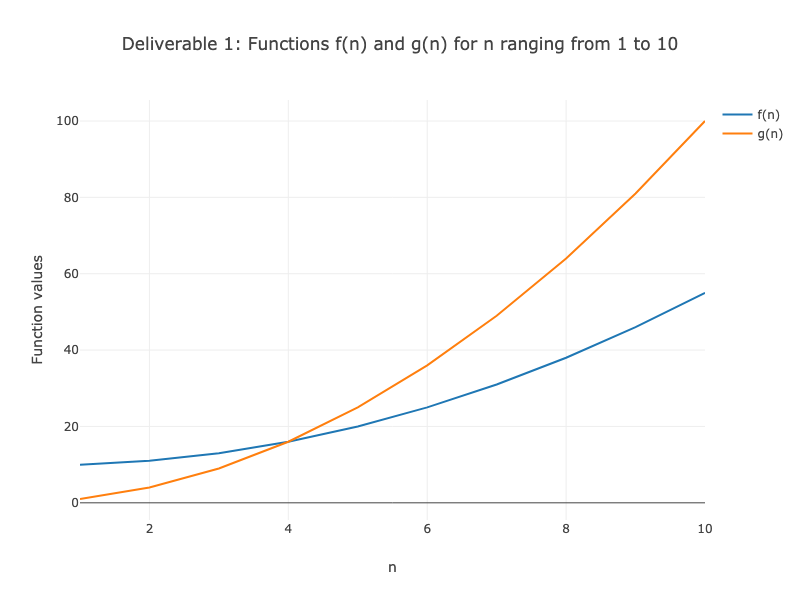
\includegraphics[width=\textwidth]{Deliverable 1: plot_1_to_10.png}
    \caption{Plot of $f(n)$ and $g(n)$ for $n$ ranging from 1 to 10.}
    \label{del1: plot_1_to_10}
\end{figure}

\begin{figure}[H]
    \centering
    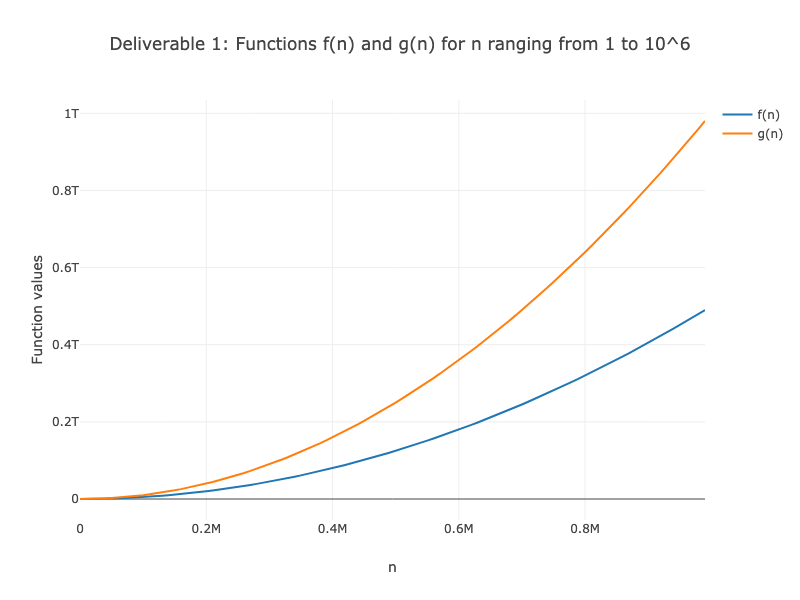
\includegraphics[width=\textwidth]{Deliverable 1: plot_1_to_1000000.png}
    \caption{Plot of $f(n)$ and $g(n)$ for $n$ ranging from 1 to $10^6$.}
    \label{del1: plot_1_to10^6}
\end{figure}

\section{Deliverable : 2(Limit Test over Deliverable 1:)}
\subsection{Functions: }
\[
    f(n) = \frac{1}{2}n(n-1) + 10, g(n) = n^2
\]

\subsection{Results of plotting and how I Interpreted them: }

I understand the limit test as how the ratio of the function scales as we approach infinity or a very large value.

\paragraph{} It is limitedly obvious in the Figure \ref{del2: plot_1_to_10} to see the curve flattening out. However, the plot of the ratio of \(f(n)\) and \(g(n)\) for \(n\) ranging from 1 to \(10^6\), as shown in Figure \ref{del2: plot_1_to10^6},
For large values of \(n\), or as \(n\) approaches infinity, the values of the ratio flattens out which means the \(\lim_{n\to \infty}   \frac{f(n)}{g(n)}\) is a positive constant indicating the same order of growth for two functions. 

\begin{figure}[H]
    \centering
    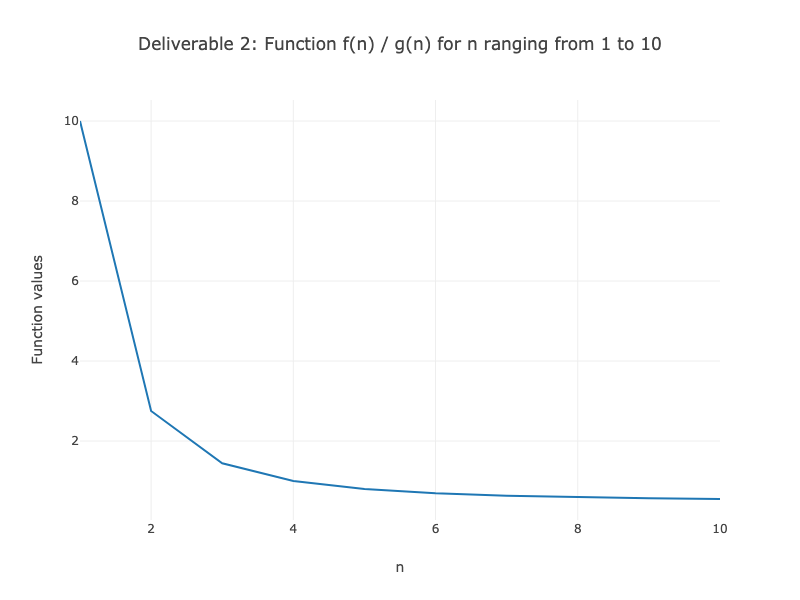
\includegraphics[width=\textwidth]{Deliverable 2: plot_1_to_10.png}
    \caption{Plot of \(\frac{f(n)}{g(n)}\) for $n$ ranging from 1 to 10.}
    \label{del2: plot_1_to_10}
\end{figure}

\begin{figure}[H]
    \centering
    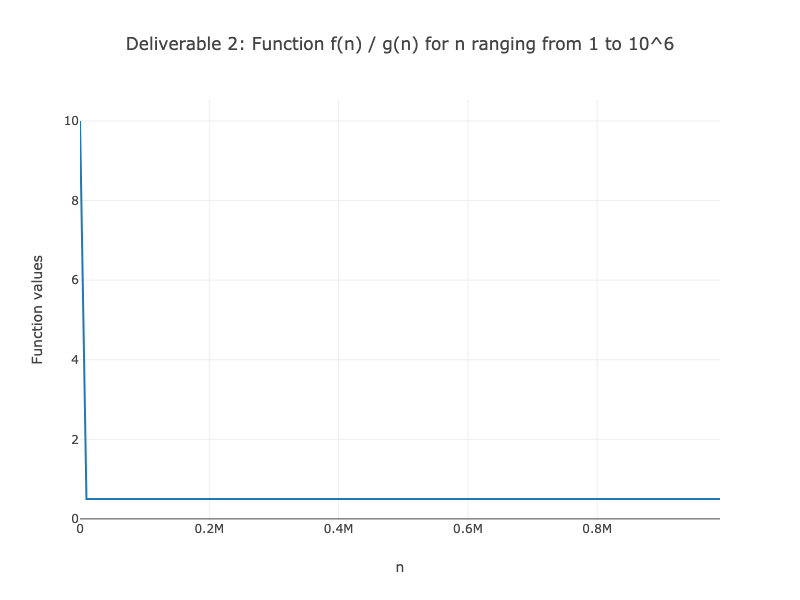
\includegraphics[width=\textwidth]{Deliverable 2: plot_1_to_1000000.png}
    \caption{Plot of \(\frac{f(n)}{g(n)}\) for $n$ ranging from 1 to $10^6$.}
    \label{del2: plot_1_to10^6}
\end{figure}

\section{Deliverable : 3}
\subsection{Functions: }
\(
    f(n) = \sqrt{n^2+3n+1} , g(n) = 5n^2
\)

\subsection{Results of plotting and how I Interpreted them: }

The function \(g(n)\) grows faster than \(f(n)\) as we can see in the Figure \ref{del3: plot_1_to_10} and Figure \ref{del3: plot_1_to10^6}.
It is not clear in the graph that has the values from \(1 to 10^6\) as I took the logarithmic scale along the axes to show the full scale.

\begin{figure}[H]
    \centering
    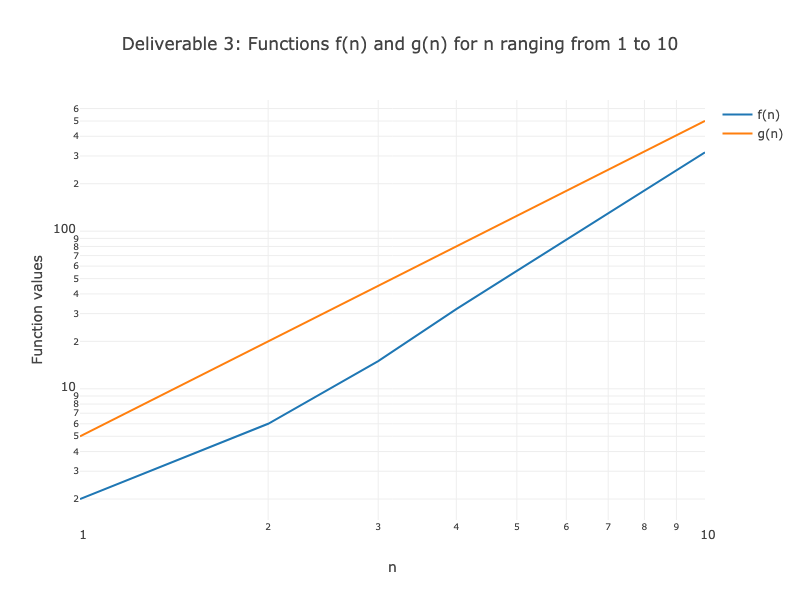
\includegraphics[width=\textwidth]{Deliverable 3: plot_1_to_10.png}
    \caption{Plot of $f(n)$ and $g(n)$ for $n$ ranging from 1 to 10.}
    \label{del3: plot_1_to_10}
\end{figure}

\begin{figure}[H]
    \centering
    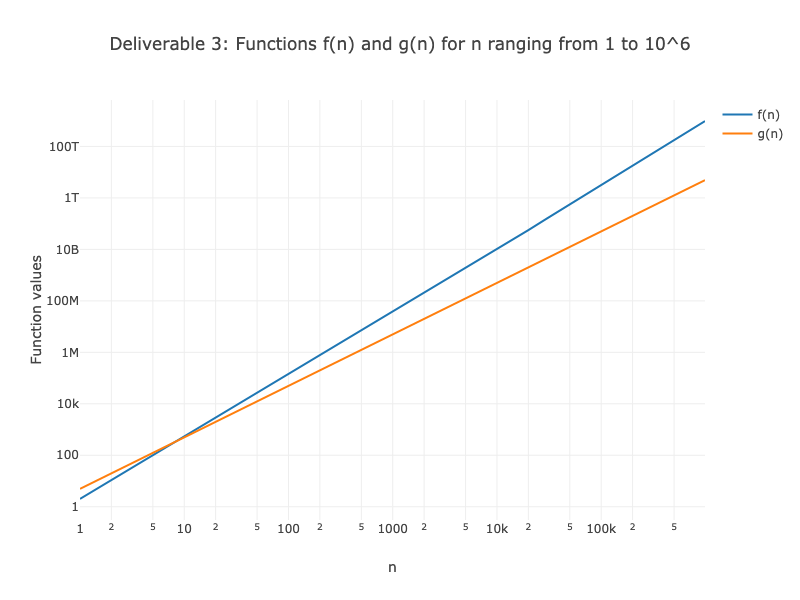
\includegraphics[width=\textwidth]{Deliverable 3: plot_1_to_1000000.png}
    \caption{Plot of $f(n)$ and $g(n)$ for $n$ ranging from 1 to $10^6$.}
    \label{del3: plot_1_to10^6}
\end{figure}

\subsection{Limit Test of Deliverable 3: }
\paragraph{} The limit test proved that the functions \(f(n)\) and \(g(n)\) have the different orders of growth. The ratio as we 
can see in the Figure \ref{del31: plot_1_to_10} and Figure \ref{del31: plot_1_to10^6}
the ratio keeps growing as the value of \(n\) increases. This indicates that the functions have different orders of growth as \(\Theta(n^{2.5}) and \Theta(n^2)\) respectively.
\begin{figure}[H]
    \centering
    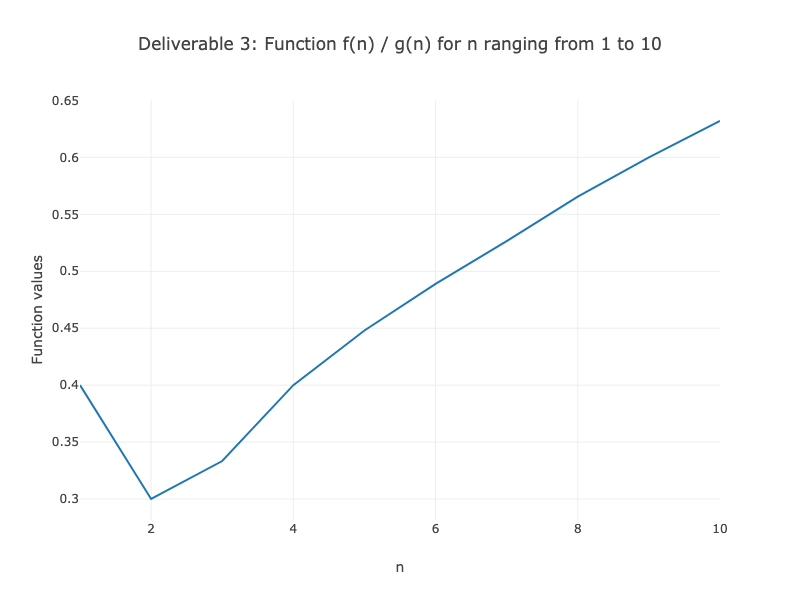
\includegraphics[width=\textwidth]{Deliverable 31: plot_1_to_10.png}
    \caption{Plot of \(\frac{f(n)}{g(n)}\) for $n$ ranging from 1 to 10.}
    \label{del31: plot_1_to_10}
\end{figure}

\begin{figure}[H]
    \centering
    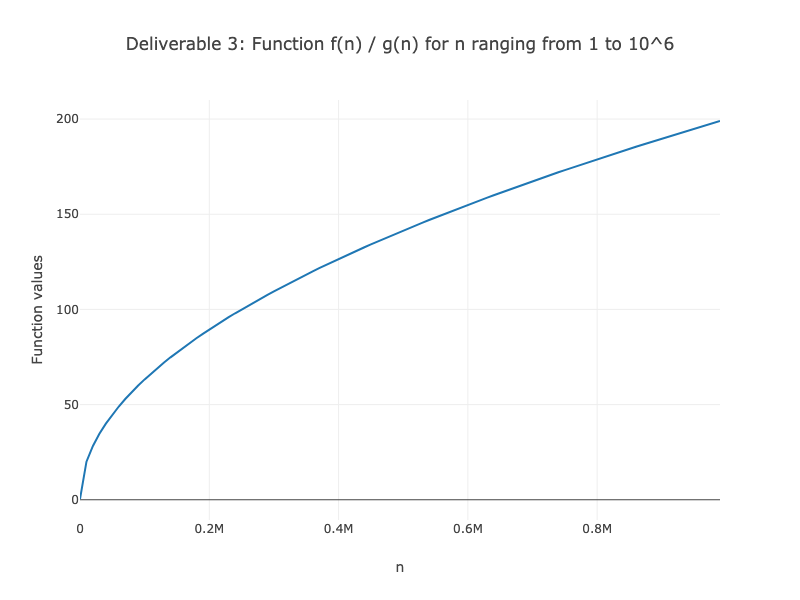
\includegraphics[width=\textwidth]{Deliverable 31: plot_1_to_1000000.png}
    \caption{Plot of \(\frac{f(n)}{g(n)}\) for $n$ ranging from 1 to $10^6$.}
    \label{del31: plot_1_to10^6}
\end{figure}

\section{Deliverable 4:}
\subsection{Functions: }
\[
    f(n) = \log(n), g(n) = \sqrt{n} 
\]

\subsection{Results of plotting and how I Interpreted them: }
Although there is a noticeble difference in the the plots of  \(f(n) and g(n)\) for smaller values of \(n\) in the Figure\ref{del4: plot_1_to_10}, we can see the difference in the growths of the fuctions for larger values of \(n\) inn the figure\ref{del4: plot_1_to10^6}
\begin{figure}[H]
    \centering
    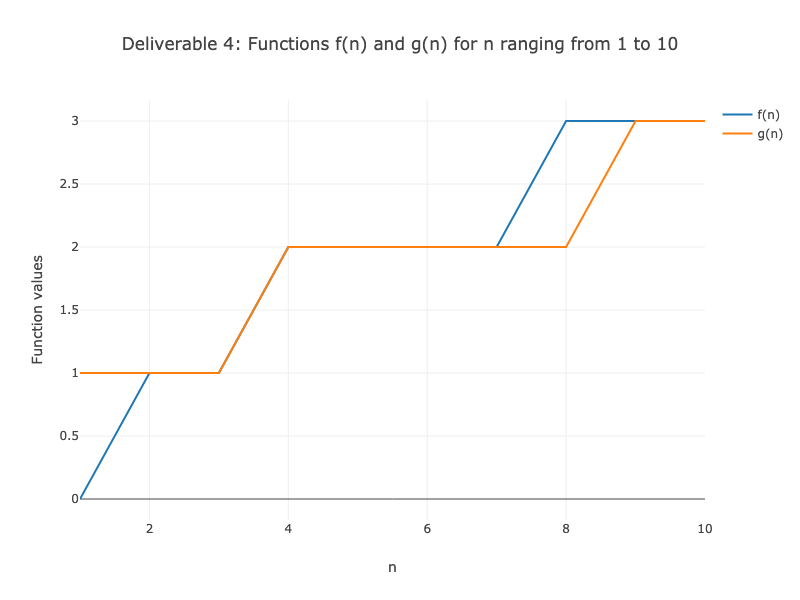
\includegraphics[width=\textwidth]{Deliverable 4: plot_1_to_10.png}
    \caption{Plot of $f(n)$ and $g(n)$ for $n$ ranging from 1 to 10.}
    \label{del4: plot_1_to_10}
\end{figure}

\begin{figure}[H]
    \centering
    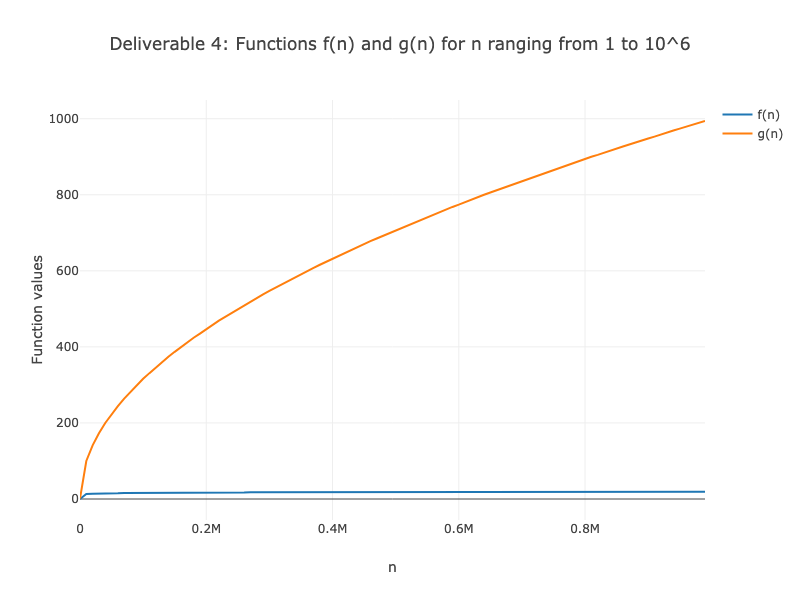
\includegraphics[width=\textwidth]{Deliverable 4: plot_1_to_1000000.png}
    \caption{Plot of $f(n)$ and $g(n)$ for $n$ ranging from 1 to $10^6$.}
    \label{del4: plot_1_to10^6}
\end{figure}

\subsection{Limit Test of Deliverable 4: }
The Limit test proves the same that the function \(f(n)\) has a significantly slower rate of growth than the function \(g(n)\), as we can see in the Figure \ref{del41: plot_1_to_10} and, very clearly, in the Figure \ref{del41: plot_1_to10^6} seems to be approaching 0 as the \(n\) tends to \(\infty\).Hence these two functions has different Orders of growth.
\begin{figure}[H]
    \centering
    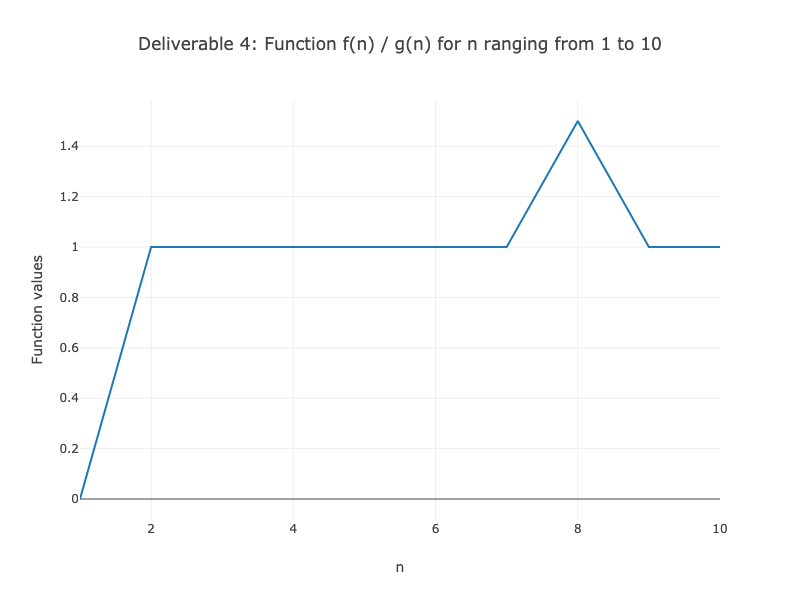
\includegraphics[width=\textwidth]{Deliverable 41: plot_1_to_10.png}
    \caption{Plot of \(\frac{f(n)}{g(n)}\) for $n$ ranging from 1 to 10.}
    \label{del41: plot_1_to_10}
\end{figure}

\begin{figure}[H]
    \centering
    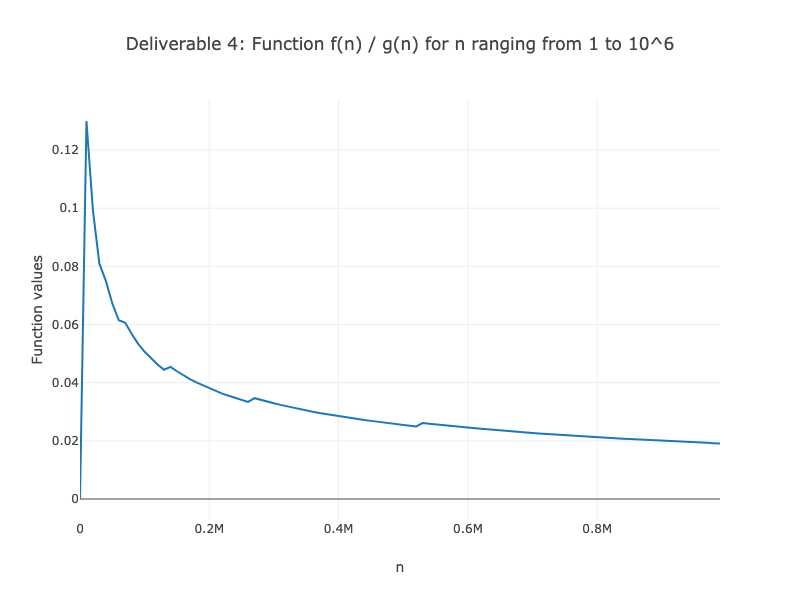
\includegraphics[width=\textwidth]{Deliverable 41: plot_1_to_1000000.png}
    \caption{Plot of \(\frac{f(n)}{g(n)}\) for $n$ ranging from 1 to $10^6$.}
    \label{del41: plot_1_to10^6}
\end{figure}

\section{Deliverable 5:}
\subsection{Functions: }
\[
    f(n) = \log_{2}{n}, g(n) = \log_{10}{n}
\]

\subsection{Results of plotting and how I Interpreted them: }
The order of growth would be confusing wiht the logarithmic functions, for smaller values of \(n\), we can see a different plots seems to be never in sync. The plots become more alike with the larger values of \(n\) as we can see in the Figure \ref{del5: plot_1_to_10} and Figure \ref{del5: plot_1_to10^6}

\begin{figure}[H]
    \centering
    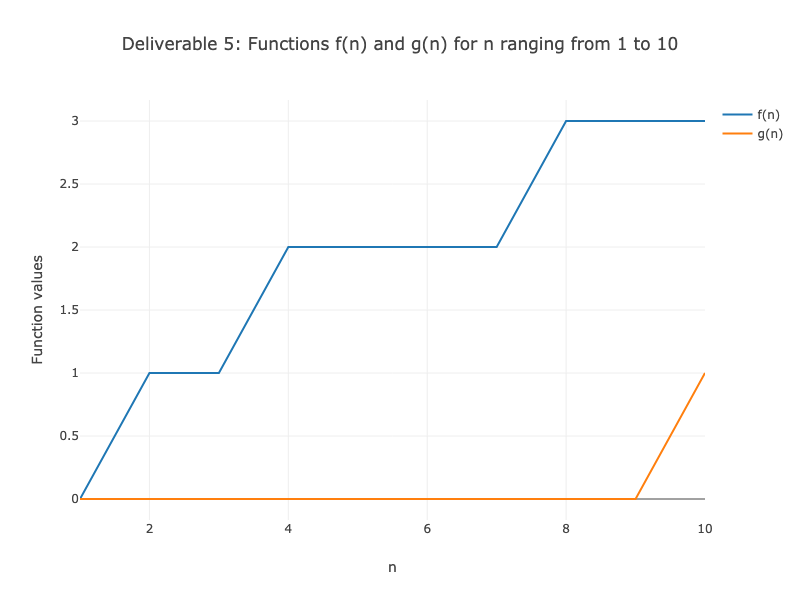
\includegraphics[width=\textwidth]{Deliverable 5: plot_1_to_10.png}
    \caption{Plot of $f(n)$ and $g(n)$ for $n$ ranging from 1 to 10.}
    \label{del5: plot_1_to_10}
\end{figure}

\begin{figure}[H]
    \centering
    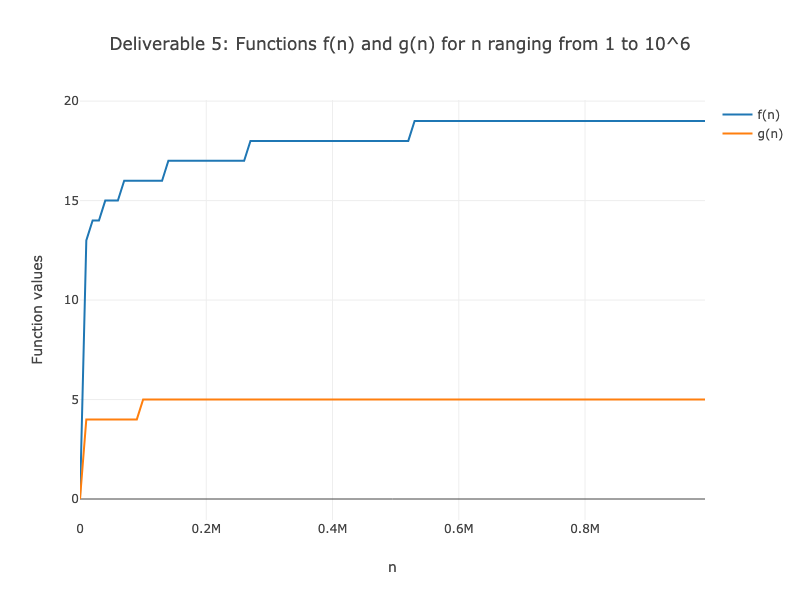
\includegraphics[width=\textwidth]{Deliverable 5: plot_1_to_1000000.png}
    \caption{Plot of $f(n)$ and $g(n)$ for $n$ ranging from 1 to $10^6$.}
    \label{del5: plot_1_to10^6}
\end{figure}

\subsection{Limit test of Deliverable 5: }
Although the plot of the ratio varies alot for the smaller values of \(n\) we can see \(n \to \infty\), the pot flattens out on some positive value which indicates that \(f(n) and g(n)\) has the same order of growth. 
\begin{figure}[H]
    \centering
    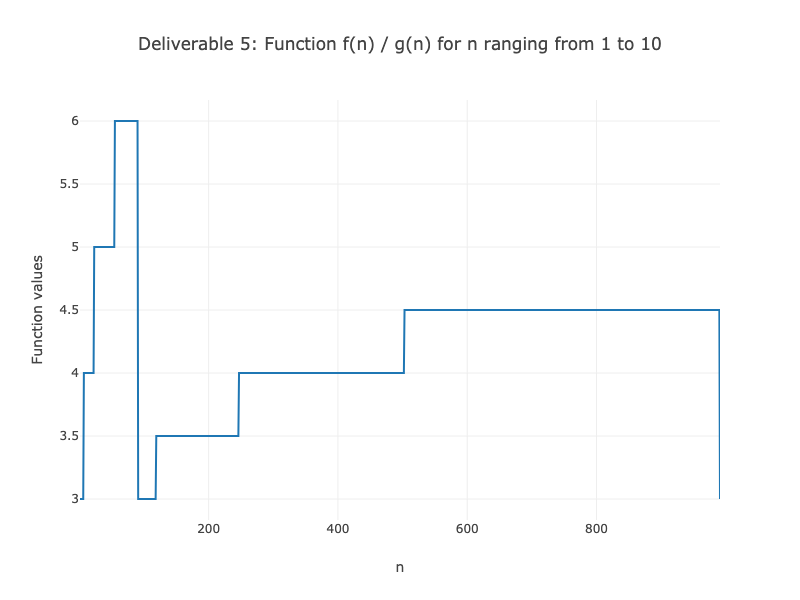
\includegraphics[width=\textwidth]{Deliverable 51: plot_1_to_1000.png}
    \caption{Plot of \(\frac{f(n)}{g(n)}\) for $n$ ranging from 1 to 10.}
    \label{del51: plot_1_to_10}
\end{figure}

\begin{figure}[H]
    \centering
    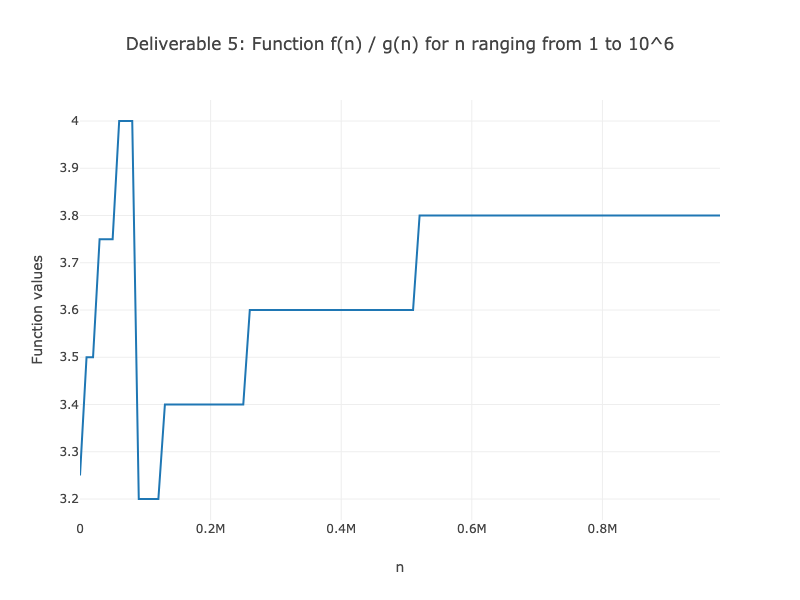
\includegraphics[width=\textwidth]{Deliverable 51: plot_1_to_1000000.png}
    \caption{Plot of \(\frac{f(n)}{g(n)}\) for $n$ ranging from 1 to $10^6$.}
    \label{del51: plot_1_to10^6}
\end{figure}

\end{document}